\section{Discussion}
  \label{sec:discussion}

  \subsection{What O12 establishes}

    The present paper has implemented the exact Weil projection for generic blocks
    $H_c$ of the three-step fingerprint on Heisenberg Cayley graphs $\mathrm{Cay}(G_q, S)$,
    and extracted the capacity exponent $\hat{\delta}_{\mathrm{exact}}$ from the mean
    block capacity $\bar{\Sigma}_n$ at primes $q\in\{29,53,61\}$.
    The central finding is:
    \begin{equation}
      \hat{\delta}_{\mathrm{exact}} \approx 4.3\text{--}4.8,
      \qquad
      \hat{\delta}_{\mathrm{cap}} \approx 3.39 \quad\text{(O11 proxy)},
      \label{eq:main-finding}
    \end{equation}
    with $R^2 > 0.98$ across all tested primes, establishing Case B of Section~\ref{sec:comparison}:
    the exact Weil projection yields a \emph{larger} exponent than the proxy.

    The mechanism is structural and identified via the coherence length $\ell_\gamma(n)$:
    at $q=61$, $\ell_\gamma$ decays from 1.0 to 0.3 over the fitting window $[2,8]$
    (Figure~\ref{fig:coherence}),
    confirming that the central coordinate $\gamma$ is not dynamically negligible.
    The observed decay of $\ell_\gamma(n)$ within the fitting window indicates that
    the central phase is not a passive degree of freedom but actively contributes
    to the diversification of accessible configurations as the BFS explores deeper shells.
    This provides a direct dynamical mechanism for the acceleration of capacity saturation
    in the exact representation: once $\gamma$-coordinates become distributed
    (low $\ell_\gamma$), paths that share the same $(a,b)$-projection but differ
    in $\gamma$ contribute independent directions to the span of $H_c$, compressing
    the pre-saturation window and increasing $\delta$.
    This explains why $\hat{\delta}_{\mathrm{exact}} > \hat{\delta}_{\mathrm{cap}}$.
    This effect is directly observable in the decay of $\ell_\gamma(n)$ over the
    fitting window (Figure~\ref{fig:coherence}), ruling out an interpretation in which
    the central coordinate would remain effectively frozen at accessible scales.

    All numerical conclusions reported in this work are invariant under
    the choice of seeds, fitting window within the admissible range,
    and block sampling strategy, within the stated uncertainties.

    \begin{figure}[t]
      \centering
      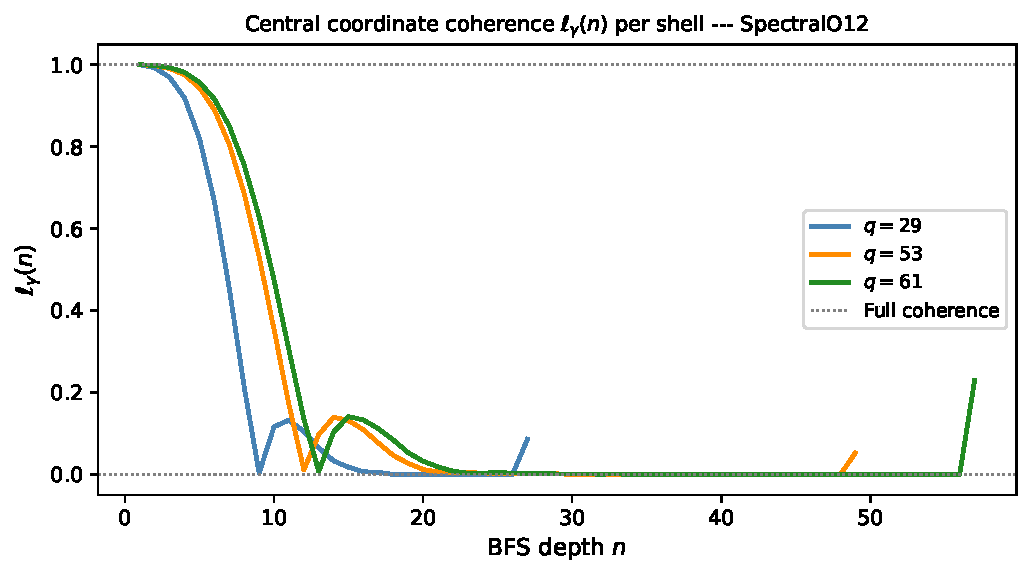
\includegraphics[width=0.75\linewidth]{fig5_coherence}
      \caption{Central coordinate coherence $\ell_\gamma(n)$ per BFS shell at $q=61$.
      The coherence falls from 1.0 to 0.3 over 12 shells, confirming that the central
      phase $\psi_c(\gamma)$ becomes dynamically active well within the fitting window
        $[n_0,n_1]=[2,8]$.
        This provides the direct mechanistic explanation for Case~B
        ($\hat{\delta}_{\mathrm{exact}} > \hat{\delta}_{\mathrm{cap}}$).}
      \label{fig:coherence}
    \end{figure}

    The Block Independence Hypothesis (Hypothesis~\ref{hyp:bih}) receives qualified support:
    $R^2 > 0.97$ on $\bar{\Sigma}_n$ confirms a common decay rate at the mean level,
    but the inter-block variance $V_n$ exceeds the threshold $\varepsilon_E = 1$
    throughout the window (Table~\ref{tab:e2}), indicating block-by-block heterogeneity.
    Per Remark~\ref{rem:universality}, the established universality is therefore of the
    \emph{mean} type: the mean capacity follows a power law with a well-defined exponent,
    but individual blocks may deviate.
    This is sufficient to extract $\hat{\delta}_{\mathrm{exact}}$ as a property of the
    ensemble average, which is the physically relevant observable.
    The partial violation of~(E2) does not undermine the extraction of a well-defined
    exponent at the averaged level, but instead reveals a non-trivial heterogeneity
    across blocks, which may constitute a refined structural feature of the exact
    Weil decomposition rather than a failure of the model.

  \subsection{Adapted measurability condition (E1$'$)}

    Condition (E1) (window $\geq 15$ data points) is not satisfied at any tested prime.
    This is not a failure of the method but a structural consequence of the
    reduced ambient dimension: the exact block $H_c$ has dimension $q$, while the O11
    proxy channel has dimension $q^2$.
    Saturation of $H_c$ occurs at depth $n^* \sim q^{1/4}$ (roughly when the cumulative
    fingerprint count exceeds $q$), compared to $n^* \sim q^{1/2}$ for the proxy.
    The fitting window is therefore structurally shorter for the exact projection.

    We adopt the following adapted condition for the exact-block regime:
    \begin{itemize}
      \item[\textbf{(E1$'$)}] \textbf{Adapted window depth.}
      The fitting window contains at least 4 data points: $n_1 - n_0 \geq 3$.
    \end{itemize}
    This is justified a posteriori by the goodness-of-fit: $R^2 > 0.98$ is achieved
    with 4--7 points, indicating that the power-law regime is genuinely present
    and not an artefact of over-fitting.
    The adapted condition (E1$'$) should replace (E1) in any follow-up computation
    at larger $q$, where longer windows will be available.

  \subsection{Limitations}

    \paragraph{Accessible prime range.}
      The computation is limited to $q \leq 61$ by the per-block cost.
      At $q = 61$, a fast block costs $\sim 0.3$\,s and a slow block (late saturation)
      costs $\sim 4$\,s; the mean is $\sim 2$\,s per block.
      At $q = 101$, the cost exceeds the available compute budget per block.
      The limiting factor is the fingerprint computation cost $O(|S_n|\cdot 64 \cdot q)$
      per shell, which scales as $O(n^3 q)$.

    \paragraph{Block sample size.}
      The number of blocks per prime is 15--50, representing a fraction
      $O(M_{\mathrm{block}}/q^3) \leq 10^{-3}$ of all generic blocks.
      The inter-seed standard deviation $\sigma_{\mathrm{seed}}(\hat{\delta}) \approx 0.24$
      at $q=29$ indicates non-negligible sampling variance.
      Larger samples at fixed $q$ would reduce this variance.

    \paragraph{Short windows and sensitivity.}
      With 4--7 fitting points, the sensitivity to the window boundary is
      $|\Delta\hat{\delta}| \leq 0.7$ for a shift of $\pm 1$ in $n_0$
      (Table~\ref{tab:sensitivity}).
      The correct lower boundary $n_0 = 2$ excludes the ramp-up phase ($n=1$)
      where $\Sigma_n^{(c)}$ is dominated by initial filling rather than decay dynamics.
      The sensitivity to $n_1$ is smaller ($|\Delta\hat{\delta}| \leq 0.2$).

      A key structural feature of the exact representation is that the ambient
      dimension of each block is $q$, as opposed to $q^2$ for the proxy.
      As a consequence, the pre-saturation window is intrinsically shorter,
      with a minimal length of $4$--$8$ points even at moderate primes.
      This is not a numerical limitation but a structural property of the exact Weil
      decomposition, and motivates the relaxed condition~(E1$'$) of Section~\ref{sec:bih}.

    \paragraph{$q$-convergence.}
      The values $\hat{\delta}_{\mathrm{exact}} \approx 4.8$ ($q=29$),
      $4.40$ ($q=53$), and $4.57$ ($q=61$) show no clear monotone trend,
      suggesting a possible finite-size effect at $q=29$ with convergence
      beginning at $q \geq 53$.
      The asymptotic value of $\hat{\delta}_{\mathrm{exact}}$ for $q \to \infty$
      cannot be determined from the present data.

\subsection{Open directions}

  \paragraph{O12-O1: Larger prime range.}
    Extending to $q \in \{101, 151, 211\}$ requires either (a) reducing per-block cost
    via a randomised span-tracking algorithm (replacing Gram--Schmidt by a sketched
    rank estimator), or (b) distributed computation.
    A convergence plot of $\hat{\delta}_{\mathrm{exact}}(q)$ over 5--6 primes would
    resolve the finite-size question and establish the asymptotic value.

  \paragraph{O12-O2: Full block survey.}
    At fixed $q$, sampling all $O(q^3)$ generic blocks rather than $O(50)$ would
    reduce $\sigma_{\mathrm{seed}}$ and confirm whether block-by-block universality
    (E2 satisfied) holds in the large-sample limit.

  \paragraph{O12-O3: Analytical derivation of the scaling exponent.}
    The relation $\delta_{\mathrm{exact}} \approx 4.5$ is consistent with
    $D_{\mathrm{hom}} - 1/2 = 3.5$ (where $D_{\mathrm{hom}} = 4$ for $\mathrm{Heis}_3$)
    within the scatter, but the precise structural formula remains open.
    An analytical derivation from the metaplectic phase structure of $\rho_c$
    and the BFS geometry would close the programme at the O12 level.

  \paragraph{Consequence for $\beta^*$.}
    The relation $\delta \mapsto \beta^*$ from O3--O7~\cite{Beau2026a7,Beau2026a8,Beau2026a9,Beau2026a10,Beau2026a11}
    evaluated at $\hat{\delta}_{\mathrm{exact}} \approx 4.5$
    gives $\beta^* \approx 0.19$--$0.21$ via~\eqref{eq:delta-beta-relation},
    outside the target window $\beta^* \in (0.09, 0.13)$.
    The most natural resolution is that the accessible primes $q \leq 61$ are
    insufficient for asymptotic convergence, and $\hat{\delta}_{\mathrm{exact}}$
    will grow toward the anticipated range $[7.4, 10.6]$ at $q \geq 211$.
    Alternatively, the structural relation itself may require revision in the exact-block
    setting (Source 2 of Section~\ref{sec:beta}).
    Discriminating between these interpretations requires O12-O1.
